The gearbox meshing system~\cite{chen2014motor} analyses the impact force and meshing time in a motor-transmission drive system,
where a shift actuator is used to switch a sleeve between gears.
%
Depending on the angular position with which the sleeve arrives at the next gear, impacts may occur which can delay the meshing process.
%
The sleeve may bounce off the gears several times before meshing succeeds.
%
The hybrid automaton model of this system consists of a \texttt{free} mode and a \texttt{meshed} mode, where the system can take circular
discrete transitions in the \texttt{free} mode corresponding to the sleeve bouncing off the sides of the gear, as well as a final transition
from the \texttt{free} mode to the \texttt{meshed} mode when meshing succeeds.
%
Resets along discrete transitions are used compute the accumulated impact impulse, which changes instantaneously whenever a transition is taken.
%
The system has five variables: two for the sleeve position and two for the sleeve velocity, and a one further variable to track the accumulated
impact impulse. 
%
The analysis goal is to find the worst-case accumulated impact impulse, as well as the longest meshing time.
%
An overview of the system is shown in Figure~\ref{fig:gb_overview}, where Figure~\ref{fig:gbo_1} shows the sleeve moving between two gears,
Figure~\ref{fig:gbo_2} shows the hybrid automaton model of the system, and Figure~\ref{fig:gbo_3} shows a simulation where the sleeve bounces off
the gear three times before meshing.

\begin{figure*}[t]
\begin{subfigure}{0.3\textwidth}
\centering
    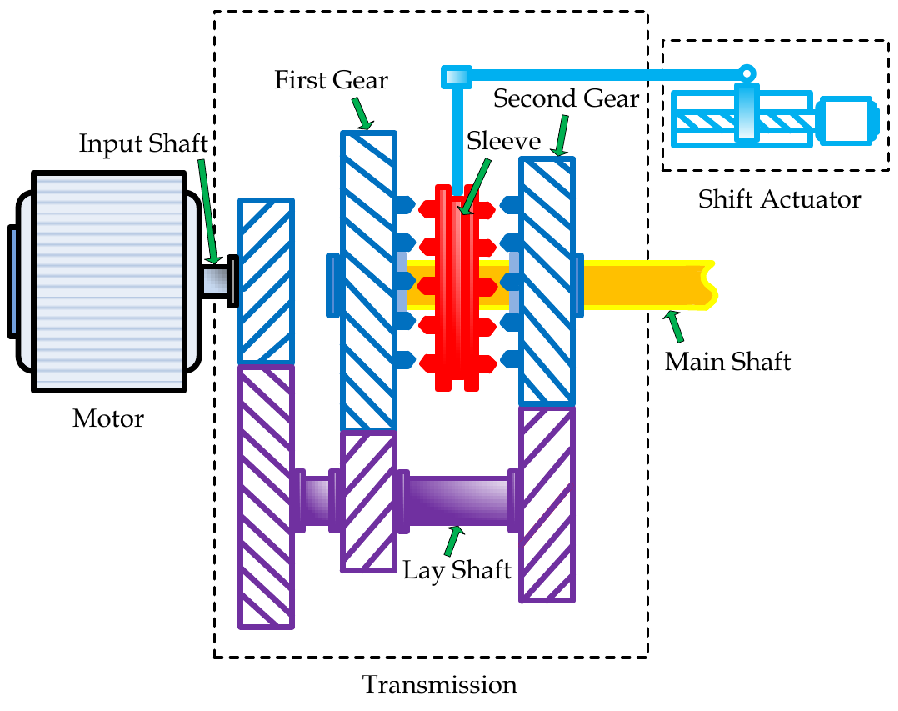
\includegraphics[width=1.0\textwidth]{images/gb_overview1.png}
    \caption{System Overview}\label{fig:gbo_1}
\end{subfigure}
\begin{subfigure}{0.3\textwidth}
\centering
    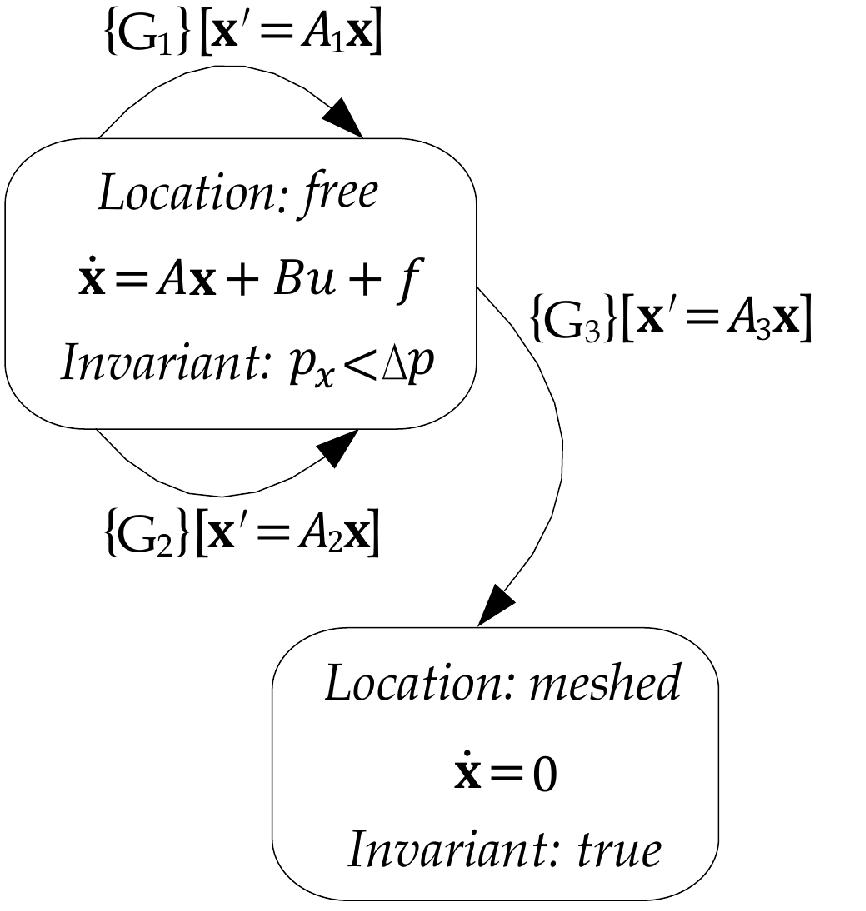
\includegraphics[width=0.7\textwidth]{images/gb_overview2.png}
    \caption{Hybrid Automaton}\label{fig:gbo_2}
\end{subfigure}
\begin{subfigure}{0.3\textwidth}
\centering
    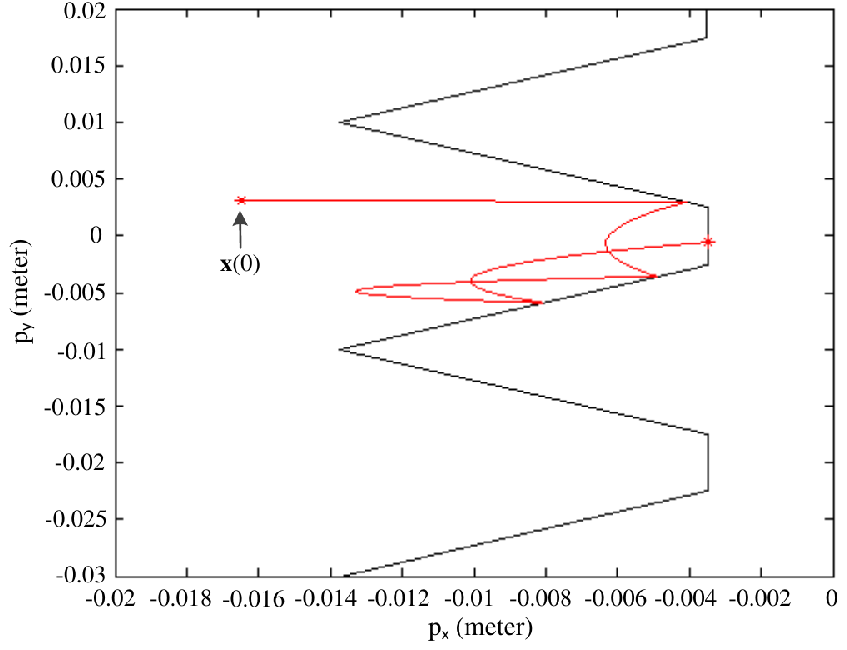
\includegraphics[width=1.0\textwidth]{images/gb_overview3.png}
    \caption{Meshing Simulation}\label{fig:gbo_3}
\end{subfigure}
\caption{Gearbox benchmark overview (images from~\cite{chen2014motor}).}\label{fig:gb_overview}
\end{figure*}

This model was also used as part of the ARCH hybrid systems verification tools competition~\cite{archcomp19}.
%
In order to make analysis tractable, a critical simplification was made: a small set of initial states was analyzed.
%
The initial set of states used for competition was so small, in fact, that all reachable states go through the
same exact sequence of discrete transitions as the simulation shown in Figure~\ref{fig:gbo_3}, with no branching possible in system executions.
%
The reason for this is that aggregation error can quickly accumulate over multiple discrete jumps, so that existing aggregation strategies
easily lead to more and more error.
%
The additional error can then make it appear that the sleeve can bounce off the gear indefinitely, without meshing.

We analyze this system using the proposed AGGDAG and deaggregation approach with a significantly larger set of initial states.
%
While the competition benchmark used the initial set of positions $x_0 \in [-0.0168, -0.0166]$, $y_0 \in [0.0029, 0.0031]$, we
analyze the larger initial set $x_0 \in [-0.017, -0.016]$, $y_0 \in [-0.005, 0.005]$.
%
We use a step size of 0.001 and analyze up to a time bound of 0.35, which is sufficient for all executions to reach the \texttt{meshed} mode,
as we will demonstrate with reachability analysis.
%
One hundred simulations from random initial states are shown in Figure~\ref{fig:gearbox_sim}, which show that many different
sequences of discrete transitions are possible. Some executions immediately mesh, while others bounce several times before meshing.

\begin{figure}[t]
\centerline{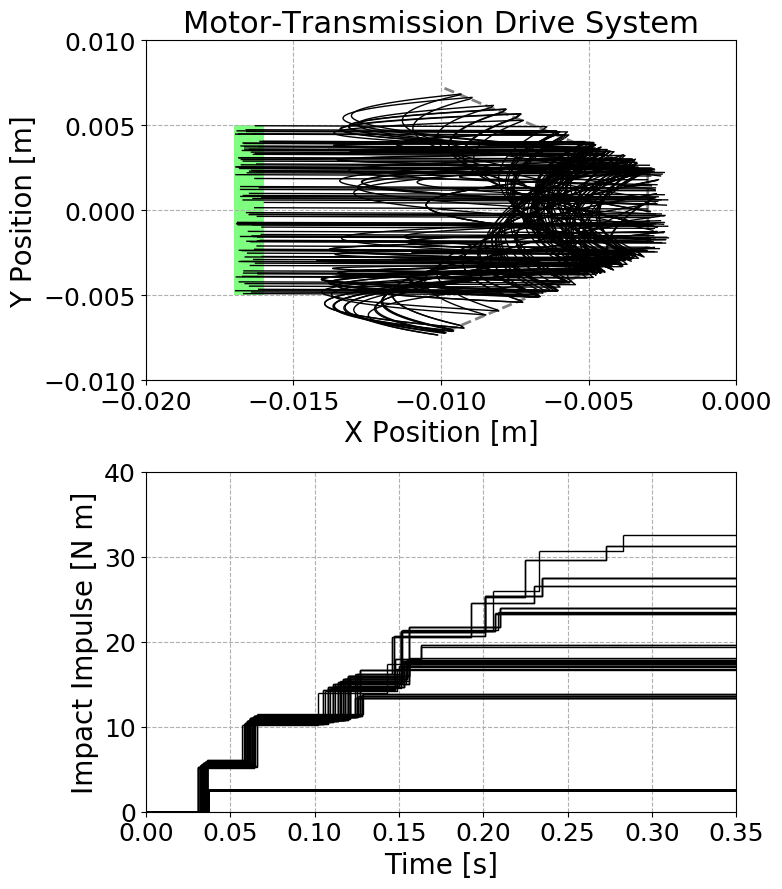
\includegraphics[width=0.8\columnwidth]{images/gearbox_sim.png}}
\caption{One hundred random simulations are shown for the gearbox system on the x/y plane (top), as well as the total impact impulse over time (bottom).
%
Notice the worst-case accumulated impact impulse, shown in Figure~\ref{fig:gearbox_reach}, was not observed in this simulation batch,
demonstrating that simulations can miss important system behaviors.
%
A video of the simulations is online at \url{https://gofile.io/?c=ypzXbv}.}
\label{fig:gearbox_sim}
\end{figure}

Since we do not have an unsafe set of states in this system, we instead drive the deaggregation process based on splits in the discrete state
transition graph.
%
That is, if a single aggregated star can reach multiple guards when computing the reach set of the dynamical system in a single mode, then we will
perform deaggregation.
%
This is done by modifying line~\ref{ln:deagg} in Algorithm~\ref{alg:aggdeagg}.
%
This use of deaggregation ensures that error from aggregation cannot introduce any spurious discrete transition sequences.

The reachable set computed by the approach is shown in Figure~\ref{fig:gearbox_reach}.
%
The worst-case meshing time is computed to be around 0.31 seconds, with a worst-case impact impulse of about 35 Nm.
%
The red line on the figure shows a witness simulation that bounces seven times before completing the meshing process.
%
Notice this worst case was not observed during the random simulations performed in Figure~\ref{fig:gearbox_sim}.

\begin{figure}[t]
\centerline{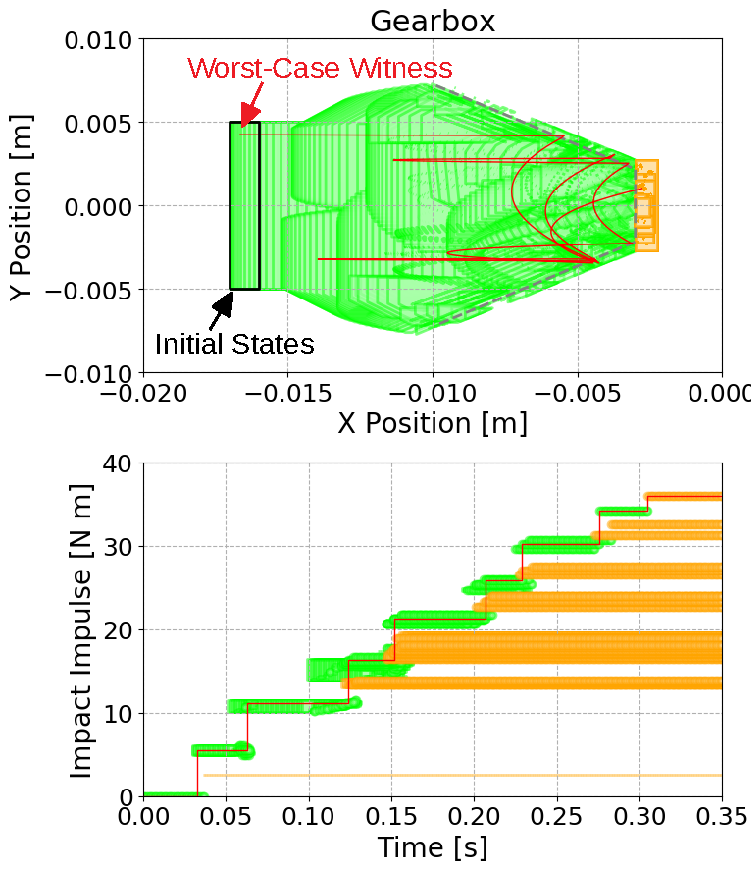
\includegraphics[width=0.8\columnwidth]{images/gearbox_annotated}}
\caption{The reachable set for the gearbox system is shown on the x/y plane (top), as well as the total impact impulse over time (bottom).
%
Green states are in the \texttt{free} mode while orange states are \texttt{meshed}.
%
The red line shows a worst-case witness which bounces seven times and reaches the maximum impact before meshing.
%
A video of the reachability computation is online at \url{https://gofile.io/?c=haaCmh}, and a video of the worst-case witness
simulation available at \url{https://gofile.io/?c=Gd5N2B}.}
\label{fig:gearbox_reach}
\end{figure}

We perform a preliminary exploration of the effects of various parameters available with our approach.
%
The results are shown in Table~\ref{tab:gearbox_params}.

\begin{table}%
  \caption{Gearbox Parameter Evaluation} \label{tab:gearbox_params}%
  \vspace{-1.0em}
\begin{tabular}{@{}lll@{}}%
\toprule%
\bf{Parameter} & \bf{Runtime (s)} & \bf{Deaggregation Steps} \\%
\midrule%
Deagg Leaves First & 17.6 & 52 \\
Deagg Root First & 11.2 & 35 \\
Deagg Most States & 16.1 & 49 \\
\hdashline[0.8pt/2pt]
Box Agg & 10.2 & 38 \\
Convex Hull Agg & \texttt{timeout} & - \\
\hdashline[0.8pt/2pt]
No Deaggregation & \texttt{timeout} & - \\
SpaceEx & \texttt{timeout} & - \\
\bottomrule
\end{tabular}%
\end{table}

For the deaggregation order exploration, we use template-based aggregation based on the mode dynamics.
%
In this case, root-first deaggregation is more efficient, both in terms of runtime and the number of deaggregation operations needed.
%
We suspect this is because overapproximation error early on in the computation leads to error later on, so even if deeaggregation is performed first on the leaves,
eventually the states closer to the root will need to be deaggregated as well.

For evaluating the aggregation method, we used root-first deaggregation.
%
There were two interesting observations.
%
First, box aggregation takes slightly less time than the default template-based aggregation, even though there are more deaggregation steps needed.
%
We attribute this speedup to the simpler star sets with the box method being easier to optimize over using an LP solver.
%
Observing the output of the reachable set, we noticed that the box method did have more error during the continuous post operation
(states to the left of the initial sets were reached when using box aggregation),
although deaggregation ensured the sequences of discrete transitions
was the same as with the more accurate template-based approach.
%
Essentially, in this case the box method was faster, but had more error.
%
Second, using the convex hull aggregation approach exceeded our one minute timeout.
%
This was because although the method from Section~\ref{sec:convexhullAgg} provide the exact convex hull, the number of variables and constraints
in result of aggregating two stars is proportional to the sums of variables and constraints in the component stars.
%
This makes the LPs grow larger in size, thus slowing the method down.
%
In this case, the result will be more accurate, but the method is slower.

Finally, we compared with existing approaches.
%
Using no deaggregation (complete aggregation), the method reached the timeout.
%
Observing the visualization we could see the suspected effect that aggregation error was growing across each jump, and
the additional error caused the sleeve to appear to be able to bounce off the gear indefinitely, without meshing.
%
With SpaceEx, we used the same settings as was used in the ARCH hybrid systems tools competition~\cite{archcomp19},
changing only the initial set of states.
%
By limiting the maximum number of discrete transitions and observing the output,
we could observe the same effect; the reachable states was growing as more and more discrete transition were processed, which
gave the appearance it was possible for the sleeve to bounce indefinitely without meshing.

% leaves-first: 17.6, 52 deaggs
% root-first: 11.2, 35 deaggs
% most states: 16.1, 49 deaggs
%
% box agg: 10.2, 38 deaggs
% chull-agg: timeout
% full-agg: timeout
% spaceex: timeout
